\documentclass[tikz,border=10pt]{standalone}
\usepackage{tikz}
\usetikzlibrary{shapes,arrows,positioning,calc,decorations.pathmorphing,backgrounds,shadows,fit,matrix}

% Define colors
\definecolor{primaryblue}{RGB}{0,102,204}
\definecolor{secondarygreen}{RGB}{46,204,113}
\definecolor{accentorange}{RGB}{255,127,0}
\definecolor{warningred}{RGB}{231,76,60}
\definecolor{lightgray}{RGB}{236,240,241}
\definecolor{darkgray}{RGB}{52,73,94}

\begin{document}
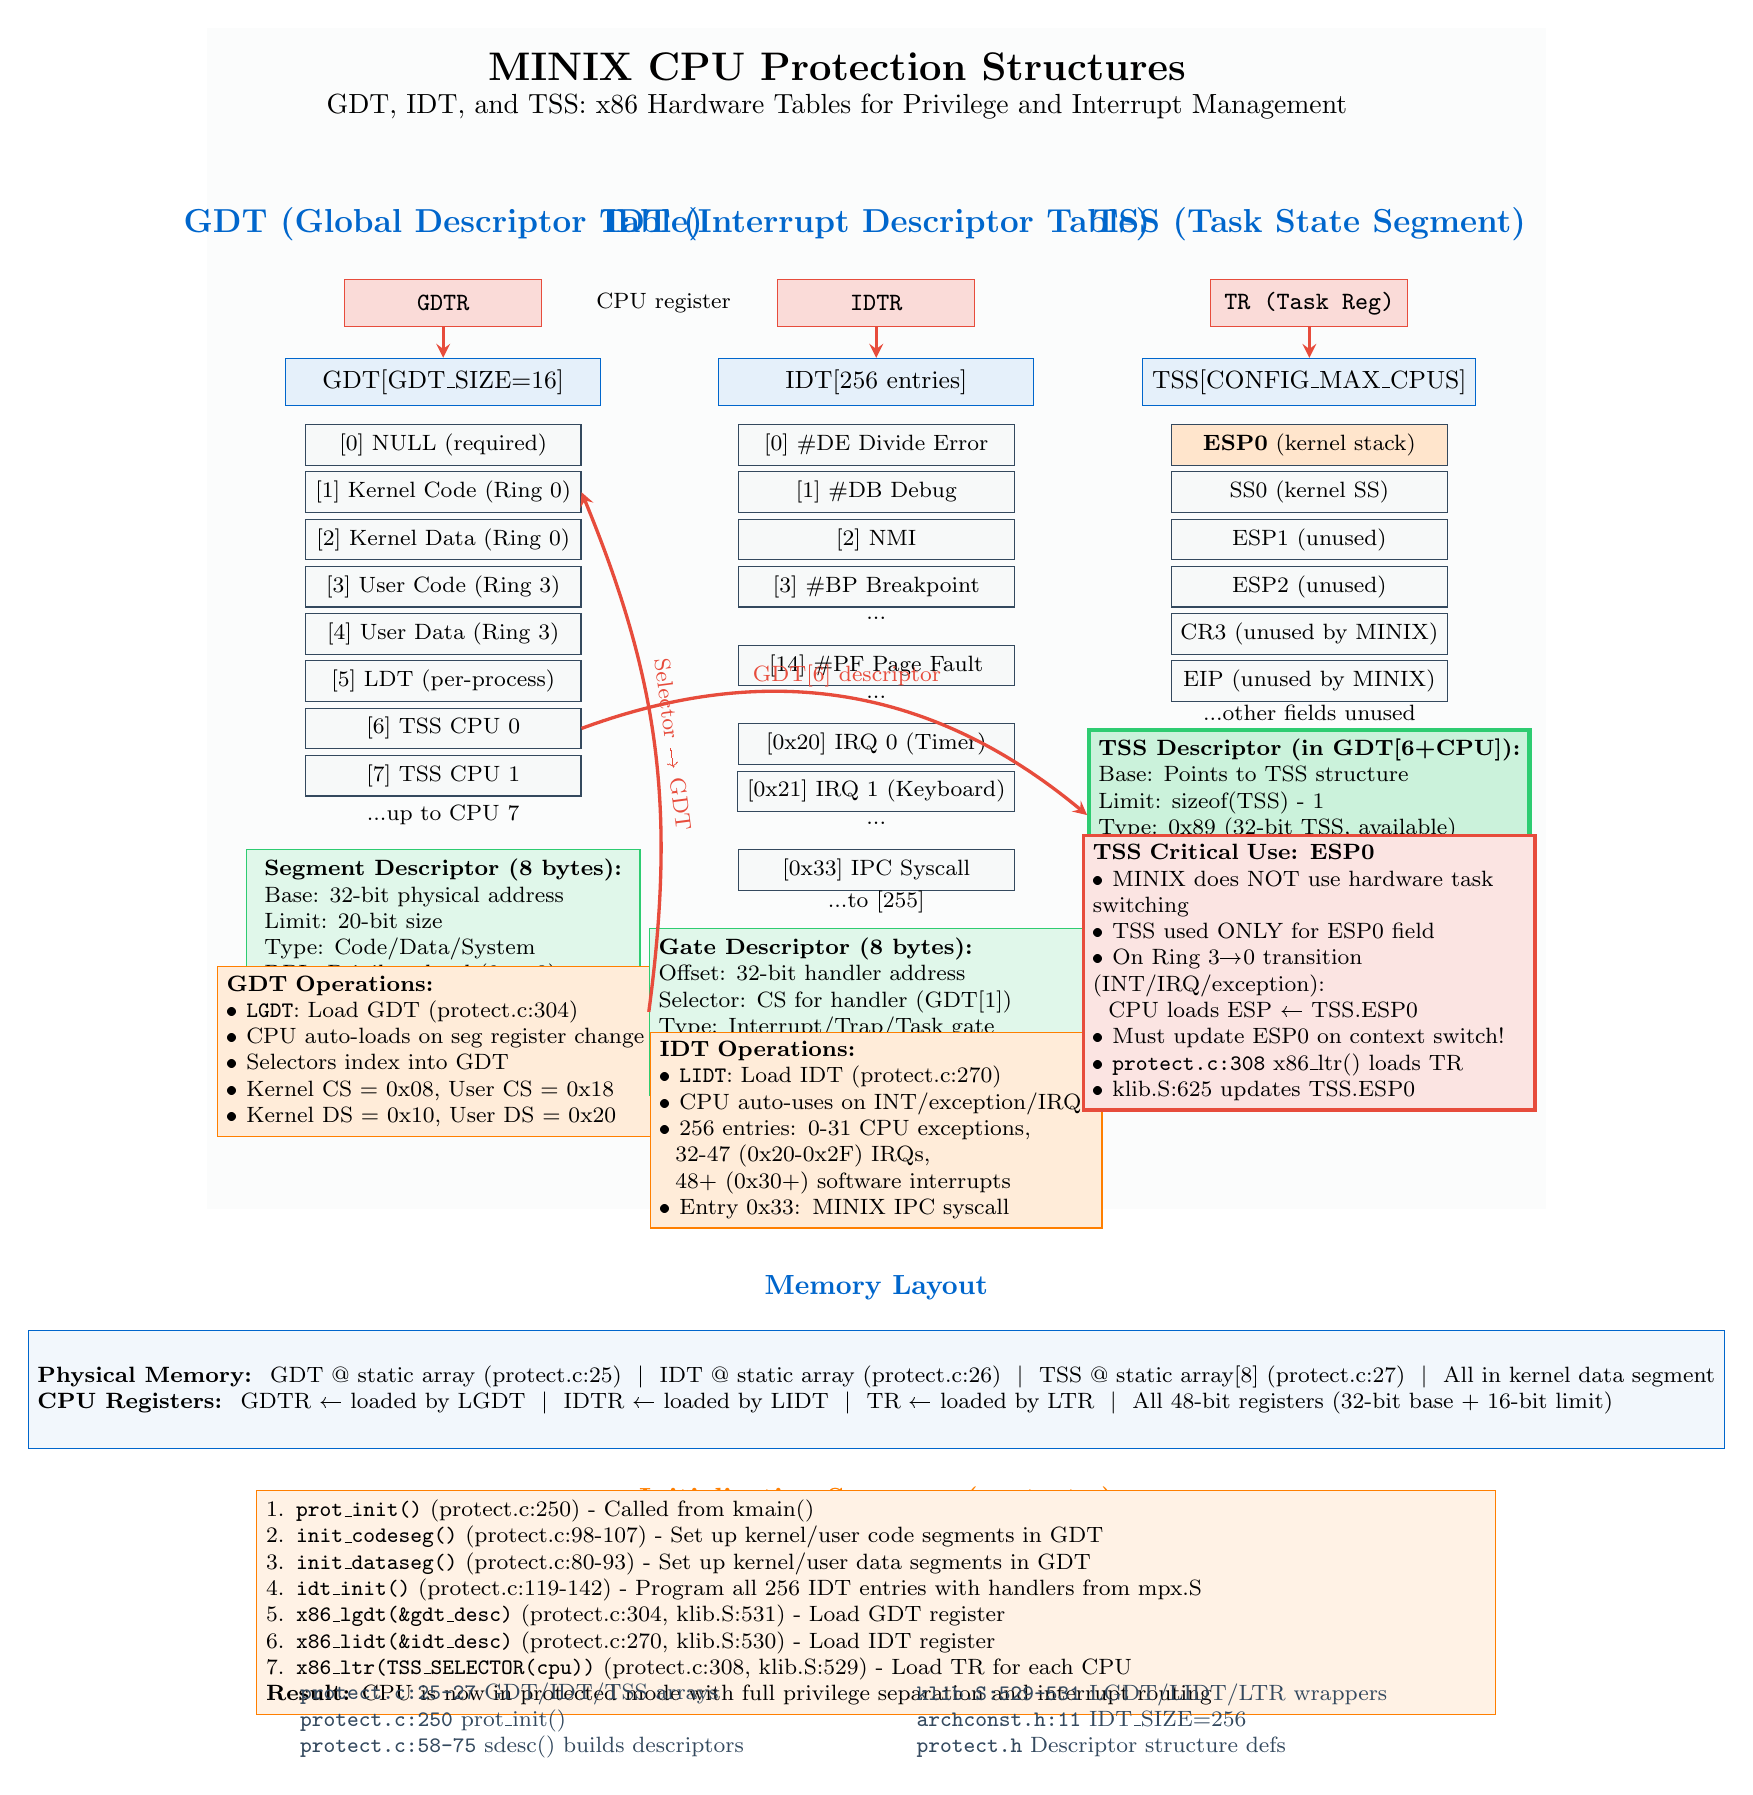
\begin{tikzpicture}[
    table/.style={rectangle, draw=primaryblue, fill=primaryblue!10, minimum width=4cm, minimum height=0.6cm, font=\small, align=center},
    entry/.style={rectangle, draw=darkgray, fill=lightgray!40, minimum width=3.5cm, minimum height=0.5cm, font=\footnotesize, align=left},
    descriptor/.style={rectangle, draw=secondarygreen, fill=secondarygreen!15, minimum width=5cm, minimum height=1.2cm, font=\footnotesize, align=left},
    register/.style={rectangle, draw=warningred, fill=warningred!20, minimum width=2.5cm, minimum height=0.6cm, font=\small\ttfamily, align=center},
    arrow/.style={->, >=stealth, thick},
    ptr/.style={arrow, warningred, line width=1.2pt},
    label/.style={font=\footnotesize}
]

% Title
\node[font=\Large\bfseries] at (8, 17) {MINIX CPU Protection Structures};
\node[font=\normalsize] at (8, 16.5) {GDT, IDT, and TSS: x86 Hardware Tables for Privilege and Interrupt Management};

%% GDT (Global Descriptor Table)
\node[font=\bfseries\large, primaryblue] at (3, 15) {GDT (Global Descriptor Table)};

% GDTR register
\node[register] (gdtr) at (3, 14) {GDTR};
\node[label] at (5.8, 14) {CPU register};

% GDT structure
\node[table] (gdt_header) at (3, 13) {GDT[GDT\_SIZE=16]};

\node[entry] (gdt0) at (3, 12.2) {[0] NULL (required)};
\node[entry] (gdt1) at (3, 11.6) {[1] Kernel Code (Ring 0)};
\node[entry] (gdt2) at (3, 11.0) {[2] Kernel Data (Ring 0)};
\node[entry] (gdt3) at (3, 10.4) {[3] User Code (Ring 3)};
\node[entry] (gdt4) at (3, 9.8) {[4] User Data (Ring 3)};
\node[entry] (gdt5) at (3, 9.2) {[5] LDT (per-process)};
\node[entry] (gdt6) at (3, 8.6) {[6] TSS CPU 0};
\node[entry] (gdt7) at (3, 8.0) {[7] TSS CPU 1};
\node[label] at (3, 7.5) {...up to CPU 7};

% GDT descriptor details
\node[descriptor] (gdt_desc) at (3, 6) {
\textbf{Segment Descriptor (8 bytes):}\\
Base: 32-bit physical address\\
Limit: 20-bit size\\
Type: Code/Data/System\\
DPL: Privilege level (0 or 3)\\
Present: 1 bit
};

% Pointer from GDTR
\draw[ptr] (gdtr) -- (gdt_header);

% GDT operations
\node[font=\footnotesize, fill=accentorange!15, draw=accentorange, text width=5.5cm, align=left] at (3, 4.5) {
\textbf{GDT Operations:}\\
• \texttt{LGDT}: Load GDT (protect.c:304)\\
• CPU auto-loads on seg register change\\
• Selectors index into GDT\\
• Kernel CS = 0x08, User CS = 0x18\\
• Kernel DS = 0x10, User DS = 0x20
};

%% IDT (Interrupt Descriptor Table)
\node[font=\bfseries\large, primaryblue] at (8.5, 15) {IDT (Interrupt Descriptor Table)};

% IDTR register
\node[register] (idtr) at (8.5, 14) {IDTR};

% IDT structure
\node[table] (idt_header) at (8.5, 13) {IDT[256 entries]};

\node[entry] (idt0) at (8.5, 12.2) {[0] \#DE Divide Error};
\node[entry] (idt1) at (8.5, 11.6) {[1] \#DB Debug};
\node[entry] (idt2) at (8.5, 11.0) {[2] NMI};
\node[entry] (idt3) at (8.5, 10.4) {[3] \#BP Breakpoint};
\node[label] at (8.5, 10.0) {...};
\node[entry] (idt14) at (8.5, 9.4) {[14] \#PF Page Fault};
\node[label] at (8.5, 9.0) {...};
\node[entry] (idt32) at (8.5, 8.4) {[0x20] IRQ 0 (Timer)};
\node[entry] (idt33) at (8.5, 7.8) {[0x21] IRQ 1 (Keyboard)};
\node[label] at (8.5, 7.4) {...};
\node[entry] (idt51) at (8.5, 6.8) {[0x33] IPC Syscall};
\node[label] at (8.5, 6.4) {...to [255]};

% IDT descriptor details
\node[descriptor] (idt_desc) at (8.5, 5) {
\textbf{Gate Descriptor (8 bytes):}\\
Offset: 32-bit handler address\\
Selector: CS for handler (GDT[1])\\
Type: Interrupt/Trap/Task gate\\
DPL: Min privilege (0 for HW, 3 for INT)\\
Present: 1 bit
};

% Pointer from IDTR
\draw[ptr] (idtr) -- (idt_header);

% IDT operations
\node[font=\footnotesize, fill=accentorange!15, draw=accentorange, text width=5.5cm, align=left] at (8.5, 3.5) {
\textbf{IDT Operations:}\\
• \texttt{LIDT}: Load IDT (protect.c:270)\\
• CPU auto-uses on INT/exception/IRQ\\
• 256 entries: 0-31 CPU exceptions,\\
\ \ 32-47 (0x20-0x2F) IRQs,\\
\ \ 48+ (0x30+) software interrupts\\
• Entry 0x33: MINIX IPC syscall
};

%% TSS (Task State Segment)
\node[font=\bfseries\large, primaryblue] at (14, 15) {TSS (Task State Segment)};

% TR register
\node[register] (tr) at (14, 14) {TR (Task Reg)};

% TSS structure (per-CPU)
\node[table] (tss_header) at (14, 13) {TSS[CONFIG\_MAX\_CPUS]};

\node[entry, fill=accentorange!20] (tss_esp0) at (14, 12.2) {\textbf{ESP0} (kernel stack)};
\node[entry] (tss_ss0) at (14, 11.6) {SS0 (kernel SS)};
\node[entry] (tss_esp1) at (14, 11.0) {ESP1 (unused)};
\node[entry] (tss_esp2) at (14, 10.4) {ESP2 (unused)};
\node[entry] (tss_cr3) at (14, 9.8) {CR3 (unused by MINIX)};
\node[entry] (tss_eip) at (14, 9.2) {EIP (unused by MINIX)};
\node[label] at (14, 8.8) {...other fields unused};

% TSS descriptor in GDT
\node[descriptor, fill=secondarygreen!25, draw=secondarygreen, line width=1.5pt] (tss_desc) at (14, 7.5) {
\textbf{TSS Descriptor (in GDT[6+CPU]):}\\
Base: Points to TSS structure\\
Limit: sizeof(TSS) - 1\\
Type: 0x89 (32-bit TSS, available)\\
DPL: 0 (kernel only)\\
Busy bit: Set by CPU on task switch
};

% Pointer from TR
\draw[ptr] (tr) -- (tss_header);

% Critical use case
\node[font=\footnotesize, fill=warningred!15, draw=warningred, text width=5.5cm, align=left, line width=1.2pt] at (14, 5.5) {
\textbf{TSS Critical Use: ESP0}\\
• MINIX does NOT use hardware task switching\\
• TSS used ONLY for ESP0 field\\
• On Ring 3→0 transition (INT/IRQ/exception):\\
\ \ CPU loads ESP ← TSS.ESP0\\
• Must update ESP0 on context switch!\\
• \texttt{protect.c:308} x86\_ltr() loads TR\\
• klib.S:625 updates TSS.ESP0
};

% GDT points to TSS
\draw[ptr, bend left=30] (gdt6.east) to node[above, label] {GDT[6] descriptor} (tss_desc.west);

%% Relationships
% GDT ← IDT relationship
\draw[ptr, bend right=15] (idt_desc.west) to node[above, label, sloped] {Selector → GDT} (gdt1.east);

% Background
\begin{scope}[on background layer]
    \fill[lightgray!20] (0, 17.5) rectangle (17, 2.5);
\end{scope}

% Memory layout diagram (bottom)
\node[font=\bfseries, primaryblue] at (8.5, 1.5) {Memory Layout};

\node[rectangle, draw=primaryblue, fill=primaryblue!5, minimum width=16cm, minimum height=1.5cm, align=left, font=\footnotesize] at (8.5, 0.2) {
\textbf{Physical Memory:} \
GDT @ static array (protect.c:25) \ $|$ \
IDT @ static array (protect.c:26) \ $|$ \
TSS @ static array[8] (protect.c:27) \ $|$ \
All in kernel data segment\\
\textbf{CPU Registers:} \
GDTR ← loaded by LGDT \ $|$ \
IDTR ← loaded by LIDT \ $|$ \
TR ← loaded by LTR \ $|$ \
All 48-bit registers (32-bit base + 16-bit limit)
};

% Initialization flow
\node[font=\bfseries, accentorange] at (8.5, -1.2) {Initialization Sequence (protect.c)};

\node[rectangle, draw=accentorange, fill=accentorange!10, text width=15.5cm, align=left, font=\footnotesize] at (8.5, -2.5) {
1. \texttt{prot\_init()} (protect.c:250) - Called from kmain()\\
2. \texttt{init\_codeseg()} (protect.c:98-107) - Set up kernel/user code segments in GDT\\
3. \texttt{init\_dataseg()} (protect.c:80-93) - Set up kernel/user data segments in GDT\\
4. \texttt{idt\_init()} (protect.c:119-142) - Program all 256 IDT entries with handlers from mpx.S\\
5. \texttt{x86\_lgdt(\&gdt\_desc)} (protect.c:304, klib.S:531) - Load GDT register\\
6. \texttt{x86\_lidt(\&idt\_desc)} (protect.c:270, klib.S:530) - Load IDT register\\
7. \texttt{x86\_ltr(TSS\_SELECTOR(cpu))} (protect.c:308, klib.S:529) - Load TR for each CPU\\
\textbf{Result:} CPU is now in protected mode with full privilege separation and interrupt routing
};

% File references
\node[font=\footnotesize, text=darkgray, align=left] at (4, -4) {
\texttt{protect.c:25-27} GDT/IDT/TSS arrays\\
\texttt{protect.c:250} prot\_init()\\
\texttt{protect.c:58-75} sdesc() builds descriptors
};

\node[font=\footnotesize, text=darkgray, align=left] at (12, -4) {
\texttt{klib.S:529-531} LGDT/LIDT/LTR wrappers\\
\texttt{archconst.h:11} IDT\_SIZE=256\\
\texttt{protect.h} Descriptor structure defs
};

\end{tikzpicture}
\end{document}
